% !TEX root = deckblatt4.tex
\section{Messung eines Sinussignales im Spektralbereich mittels FFT}

\subsection{Aufgabenstellung}
In dieser Aufgabe sollte man sich mit mit der FFT Funktion des Oszilloskops vertraut machen. Hierzu sollte ein einfaches Sinussignal in Zeit und Frequnezbereich gemessen und analysiert werden.

\subsection{Zeitbereich}

\begin{figure}[H]
 \begin{center}
  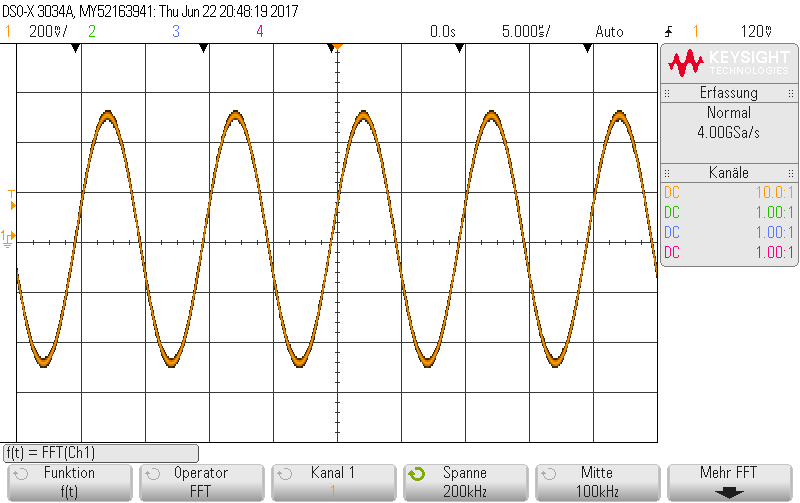
\includegraphics[height=6cm,width=12cm]{OsziBilder/bsp1_time}
 \end{center}
 \caption{Zeitverlauf des Sinussignales, $1V_{PP}$ $100kHz$}
\end{figure}

\subsection{Frequenzbereich}

\begin{figure}[H]
 \begin{center}
  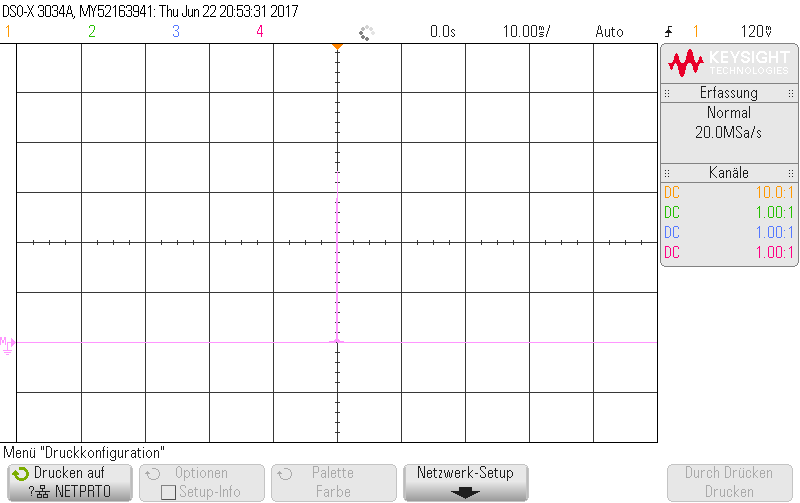
\includegraphics[height=6cm,width=12cm]{OsziBilder/bsp1_Rechteck_RMS}
 \end{center}
 \caption{Spektraldarstellung des Sinussignales, Rechteckfenster $V_{RMS}$}
\end{figure}

\begin{figure}[H]
 \begin{center}
  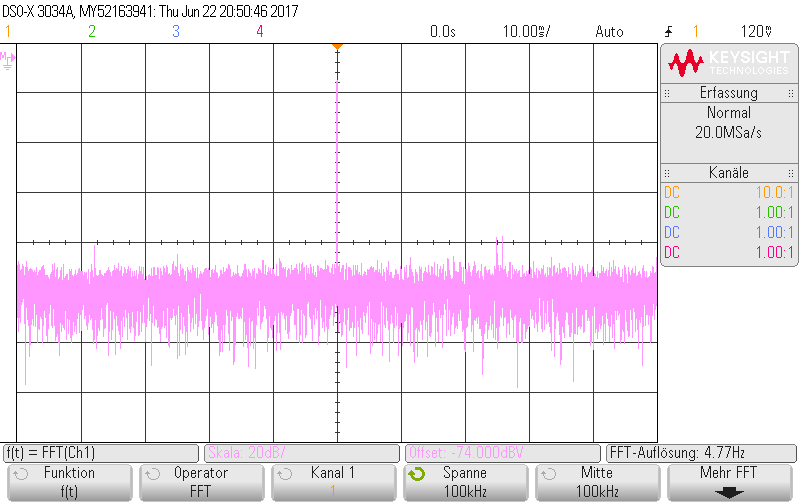
\includegraphics[height=6cm,width=12cm]{OsziBilder/bsp1_Hanning_dB}
 \end{center}
 \caption{Spektraldarstellung des Sinussignales, Hammingfenster $dBV$}
\end{figure}
\noindent
Beide Darstellungen zeigen die Spektrallinie des Sinussignales bei $1kHz$ mit einer Amplitude von $0,5V_P$. In der $dBV$-Skalierung kommen auch die Signale mit kleinerer Amplitude zur geltung, weshalb auch die Störsignale (Rauschen) zu sehen sind.\\
Um durch die FFT ein sauberes Spektrum zu erlangen, müssen verschiedene Parameter angepasst werden. So ist ist die Abtastrate (Horizontalablenkung) ausschlaggebend für die korrekte Aufzeichnung des Signales (Aliasing- Foldingeffekt). Der Frequenzbereich wird so gewählt, dass
die einezelnen Spektralkomponent gut zu erkennen sind und die benötigte Bandbreite dargestellt wird.\\

\newpage
\subsection{Fensterfunktionen}

Die Fensterfunktionen werden nach den Kriterien, minimaler Leckeffekt, Amplituden- und Frequenzgenauigkeit gewählt. Da es keine optimale Lösung gibt, die alle drei Anforderungen erfüllt, wird
die Fensterfunktion abhängig von der Problemstellung gewählt.\\
Das Oszilloskop bietet vier Verschiedenen Fensterfunktion:\\
\begin{itemize}
 \item Rechteckfenster: hoher Leckeffekt, hohe Frequenzgenauigkeit\\
 \item Hammingfenster: gut für kontinuierliche Signale\\
 \item Flache Oberseite Fenster: hohe Amplituden genauigkeit, niedrige Frequenzgenauigkeit \\
 \item Blackman-Harris-Fenster:  hohe Amplituden genauigkeit, niedrige Frequenzgenauigkeit\\
\end{itemize}
Für die weiteren Anwendungen der FFT wurde hauptsächlich das Hammingfenster verwendet, da es einen guten Kompromiss
zwischen den drei geforderten Eigenschaften darstellt.\\
